\documentclass[border=4pt]{standalone}
\usepackage{tikz}
\usetikzlibrary{arrows}
\begin{document}
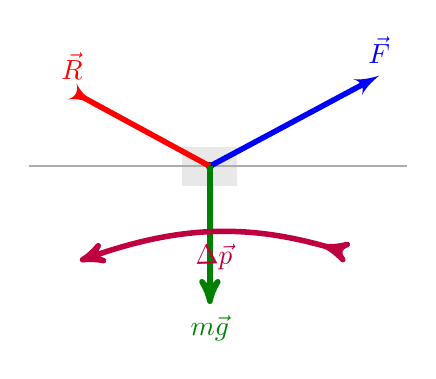
\begin{tikzpicture}
  \fill[gray!18] (-.35,-.25) rectangle (.35,.25);
  \draw[gray!65,line width=.8pt] (-2.3,0) -- (2.5,0);
  \fill (0,0) circle (1.5pt);

  \draw[blue,line width=2pt,-{latex'}] (0,0) -- (2.15,1.15) node[above] {$\vec F$};
  \draw[red,line width=2pt,-{latex' reversed}] (0,0) -- (-1.75,.95) node[above] {$\vec R$};
  \draw[green!50!black,line width=2pt,-{stealth'}] (0,0) -- (0,-1.75) node[below] {$m\vec g$};
  \draw[purple,line width=2pt,{stealth'}-{stealth' reversed}]
    (-1.65,-1.2) to[bend left=18] node[below,sloped] {$\Delta\vec p$} (1.75,-1.1);
\end{tikzpicture}
\end{document}
